\section{Results}

We report the baseline stage first (Sections IV-A and IV-B) and then the full protocol.

\subsection{Baseline: per-client Masking Gap is mostly noise}

Table~\ref{tab:baseline} compares per-client MG in the nine baseline conditions with its chance level. Average per-client MG ranges from 0.106 to 0.117, yet a model with no information about any label would score 0.103 on the same test sets. MG-excess lies between $+0.002$ and $+0.013$, about a tenth of the raw MG, and no condition differs from chance after Holm correction (smallest adjusted $p = 0.27$). Of all 540 client--seed--condition results, 8.0\% are \emph{elevated} and 1.7\% \emph{severe}, against the 5\% and 1\% that chance predicts (Fig.~\ref{fig:null}b): a small real excess may exist, but it is too small to attribute to any condition.

The simplest way to read MG would be with fixed cut-points, for example moderate at 0.10 and severe at 0.20. These sit near the median (0.10) and upper tail (95th percentile 0.13--0.24, depending on client) of the null, so they label noise as masking: under them, 52\% of the baseline results would be moderate or worse, whereas under calibrated tiers 90\% are within noise.

\begin{table}[t]
\caption{Baseline conditions compared with chance (3 seeds). MG-excess: mean over clients of MG minus its random-score null mean, with 95\% cluster-bootstrap CI. $p$: two-sided Wilcoxon test against 0, Holm-adjusted across conditions. $>$p95: share of client--seed results above their null 95th percentile (5\% expected by chance).}
\label{tab:baseline}
\centering\small
\setlength{\tabcolsep}{1.8pt}
\begin{tabular}{@{}lccrcc@{}}
\toprule
Condition & MG & Null & MG-excess [95\% CI] & $p$ & $>$p95 \\
\midrule
C1 Centralized     & 0.107 & 0.103 & $+0.004$ [$-0.007$, $0.015$] & 1.00 & 6.7\% \\
C2 Sep.\ classif.  & 0.108 & 0.103 & $+0.005$ [$-0.006$, $0.017$] & 1.00 & 6.7\% \\
C2-FL Fed.\ sep.   & 0.106 & 0.103 & $+0.002$ [$-0.011$, $0.016$] & 1.00 & 11.7\% \\
C3 FedAvg          & 0.116 & 0.103 & $+0.012$ [$0.003$, $0.022$] & 0.35 & 6.7\% \\
C4 SCAFFOLD        & 0.109 & 0.103 & $+0.006$ [$-0.004$, $0.015$] & 1.00 & 10.0\% \\
C5 CS-Agg          & 0.117 & 0.103 & $+0.013$ [$0.004$, $0.023$] & 0.27 & 11.7\% \\
C6 Ditto           & 0.113 & 0.103 & $+0.010$ [$0.000$, $0.020$] & 0.63 & 8.3\% \\
C7 q-FedAvg        & 0.113 & 0.103 & $+0.009$ [$-0.003$, $0.022$] & 1.00 & 11.7\% \\
C8 Per-dim.        & 0.111 & 0.103 & $+0.008$ [$0.000$, $0.016$] & 0.63 & 13.3\% \\
\bottomrule
\end{tabular}
\end{table}

\begin{figure}[t]
\centering
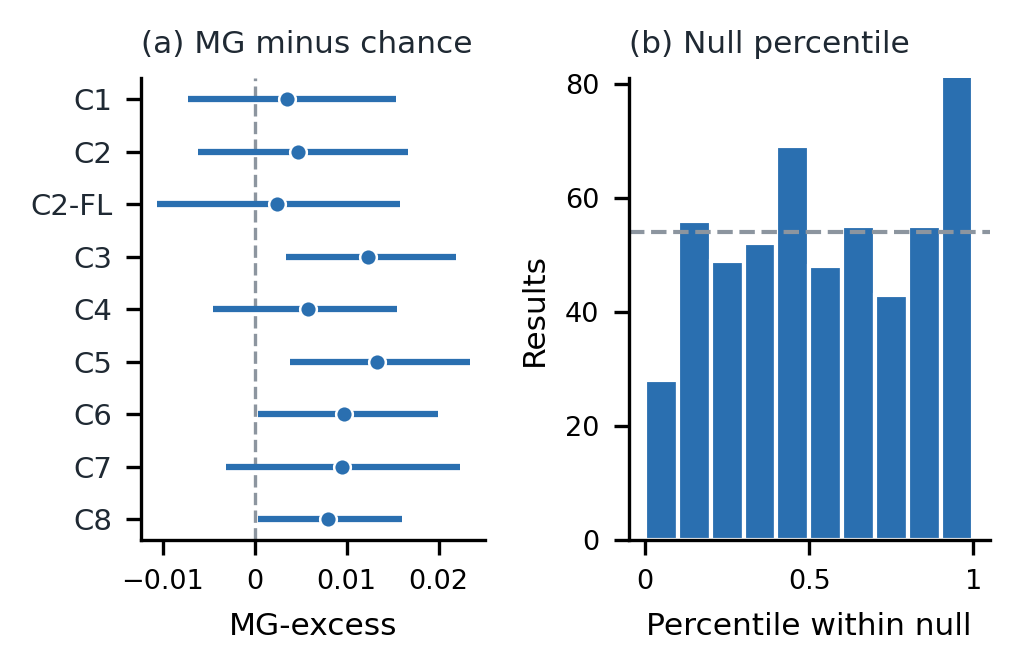
\includegraphics[width=\columnwidth]{fig11_null_calibration.png}
\caption{Null calibration of the baseline conditions (names in Table~\ref{tab:baseline}). (a) MG-excess with 95\% cluster-bootstrap CIs; dashed: chance (0). (b) Percentile of each per-client MG within its own null, for all 540 client--seed--condition results; dashed: the count expected by chance. Real masking would pile up near 1.}
\label{fig:null}
\end{figure}

\emph{Why the noise is so large.} The null 95th percentile of MG drops below 0.10 only at about 300 test records per client, and below 0.05 only above 1,000 (Fig.~\ref{fig:power}); our clients have 37--141. The minimum over seven AUCs picks whichever dimension happens to be estimated worst, which favors dimensions with few cases: 30--45\% of clients have too few Mental cases for any AUC. Which dimension is worst is only partly systematic: Sleep is the minimum in 22.0\% of results, against 16.0\% under the null. Eq.~(\ref{eq:closed}) gives 250 and 1,000 records for gaps of 0.10 and 0.05, within 12\% of the exact values (290 and 1,150).

\begin{figure}[t]
\centering
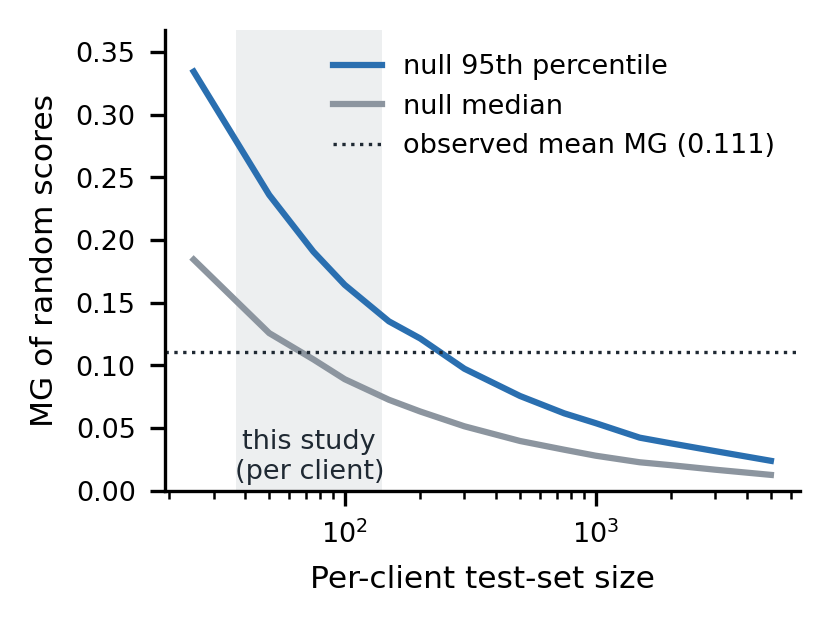
\includegraphics[width=0.82\columnwidth]{fig12_power_curve.png}
\caption{Median and 95th percentile of MG for random scores versus per-client test size, at this sample's prevalences. Shaded: the per-client test sizes in this study; dotted: mean observed MG over the baseline conditions.}
\label{fig:power}
\end{figure}

\emph{Comparing conditions.} With clients as units, no condition differs in MG from its reference: C2 versus C1, C3 versus C1, and C2-FL, C6, C7 and C8 versus C3 all have Holm $p = 1.00$ (e.g., C2-FL versus FedAvg, Hodges--Lehmann $-0.010$ [$-0.027$, $0.005$]), and the mixed model finds no condition different from FedAvg ($p \geq 0.23$). Read with fixed cut-points instead, the same numbers would label about half of all client results as masked under every method.

\subsection{Baseline population audit: federated outputs fall to chance}

Pooling clients removes most of the noise (null population MG: mean 0.027, 95th percentile 0.038). Table~\ref{tab:popauc} gives the client-averaged AUC per dimension. The centralized model is above chance on all seven dimensions (0.56--0.64). Under every federated condition, Sleep (0.49--0.52) and Mental (0.49--0.52) fall to chance, and FedAvg is above chance on only two of seven dimensions. This is a real failure of the baseline pipeline, and population MG misses it: no condition's population MG exceeds chance after Holm correction ($p \geq 0.16$; 0.033--0.043 for federated conditions), because MG measures the spread between dimensions, and when most dimensions sit near chance that spread is small. Only checking each dimension against chance finds the failure. Section~\ref{sec:full} traces it to unscaled inputs.

\begin{table}[t]
\caption{Client-averaged AUC per dimension, baseline conditions (3 seeds). $^{*}$: 95\% cluster-bootstrap CI above 0.5.}
\label{tab:popauc}
\centering\small
\setlength{\tabcolsep}{2.2pt}
\begin{tabular}{@{}lccccccc@{}}
\toprule
 & Sleep & Act. & Sed. & Ment. & Metab. & Wellb. & Diet \\
\midrule
C1    & .557$^{*}$ & .588$^{*}$ & .554$^{*}$ & .571$^{*}$ & .638$^{*}$ & .610$^{*}$ & .574$^{*}$ \\
C2    & .562$^{*}$ & .584$^{*}$ & .548$^{*}$ & .534 & .628$^{*}$ & .588$^{*}$ & .569$^{*}$ \\
C2-FL & .509 & .529$^{*}$ & .535$^{*}$ & .489 & .575$^{*}$ & .545$^{*}$ & .522$^{*}$ \\
C3    & .495 & .518 & .503 & .504 & .568$^{*}$ & .529$^{*}$ & .509 \\
C4    & .488 & .531$^{*}$ & .510 & .486 & .539$^{*}$ & .523 & .500 \\
C5    & .496 & .494 & .511 & .506 & .567$^{*}$ & .532$^{*}$ & .509 \\
C6    & .520 & .533$^{*}$ & .525 & .517 & .556$^{*}$ & .556$^{*}$ & .505 \\
C7    & .502 & .504 & .512 & .509 & .556$^{*}$ & .508 & .509 \\
C8    & .494 & .488 & .514 & .516 & .540$^{*}$ & .558$^{*}$ & .527$^{*}$ \\
\bottomrule
\end{tabular}
\end{table}
